\documentclass[../../D1.tex]{subfiles}

\begin{document}
\emph{
- Discuss VPU/TPU/APU/GPU/FPGA/ASIC memory arcitecture and how it handles matrix sparsity\\
- Show ineffectivity of pruning on hardware without optimisations for sparse matrices\\
}
%The explosion of Deep Neural Network applications in recent years has prompted the production of a wave of specialised hardware architectures to improve the efficiency and compute of these kinds of workloads. The mainstay of this form of processing has been until recently been dominated by GPUs.\\


\subsubsection{Memory Allocation}\label{sec:MemAlloc}
\begin{figure}[H]
    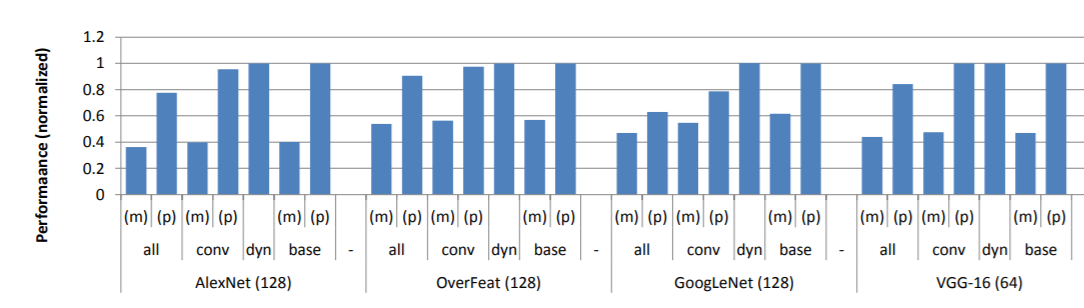
\includegraphics[width=1\textwidth]{vDNNperf.png} 
    \caption{vDNN performance, showing the throughput using various memory allocation strategies. \\ \textbf{(Adopted figure from~\autocite{rhuVDNNVirtualizedDeep2016})}}
    \label{fig:vDNNperf}   
\end{figure}
While designed specifically for training networks that would otherwise be to large for a GPU, the memory manager vDNN proposed by Rhu et al~\autocite{rhuVDNNVirtualizedDeep2016}~does provide some insight into the importance of memory locality to neural network throughput.
Fig.~\ref{fig:vDNNperf}~summarizes the performance of neural networks using vDNN to manage memory compared to a baseline memory management policy ($base$). The vDNN policies include: static policies (denoted as $all$ and $conv$) and a dynamic policy ($dyn$).
$base$ simply loads the full model into the GPU memory, consequently providing optimal memory locality. $all$ refers to a policy of moving all $X$s out of GPU memory, and $conv$ only offloads $X$s from convolutional layers, $X$s are the input matrices to each layer, denoted by the red arrows in Fig.~\ref{fig:memAllocInf}.
Each of $base$, $conv$ and $all$ are evaluated using two distinct convolutional algorithms - memory-optimal ($m$) and performance-optimal ($p$).
Finally the $dyn$ allocation policy chooses ($m$) and ($p$) dynamically at runtime.

Observing the results in Fig.~\ref{fig:vDNNperf}~a significant ($58\%$ and $55\%$) performance loss is evident compared to baseline, this loss is caused because no effort is made to optimise location of network parameters in memory. In this example the memory locality is compared between memory in the GPU (VRAM) and host memory (DRAM) accessed via the PCI lanes.

\begin{figure}[H]
    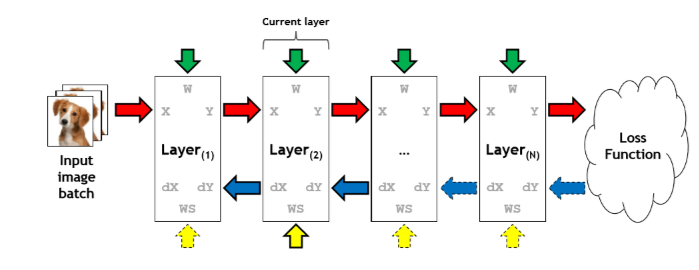
\includegraphics[width=1\textwidth]{MemoryAlloc.png} 
    \caption{Memory allocations required for linear networks. All green ($W$) and red ($X$) arrows are allocated during inference, the blue and yellow arrows are allocated during training.\\ \textbf{(Adopted figure from~\autocite{rhuVDNNVirtualizedDeep2016})}}
    \label{fig:memAllocInf}   
\end{figure}


Justifies the need for compression ... pruning


\subsubsection{Memory Access}

\begin{figure}[H]
    \begin{center}
        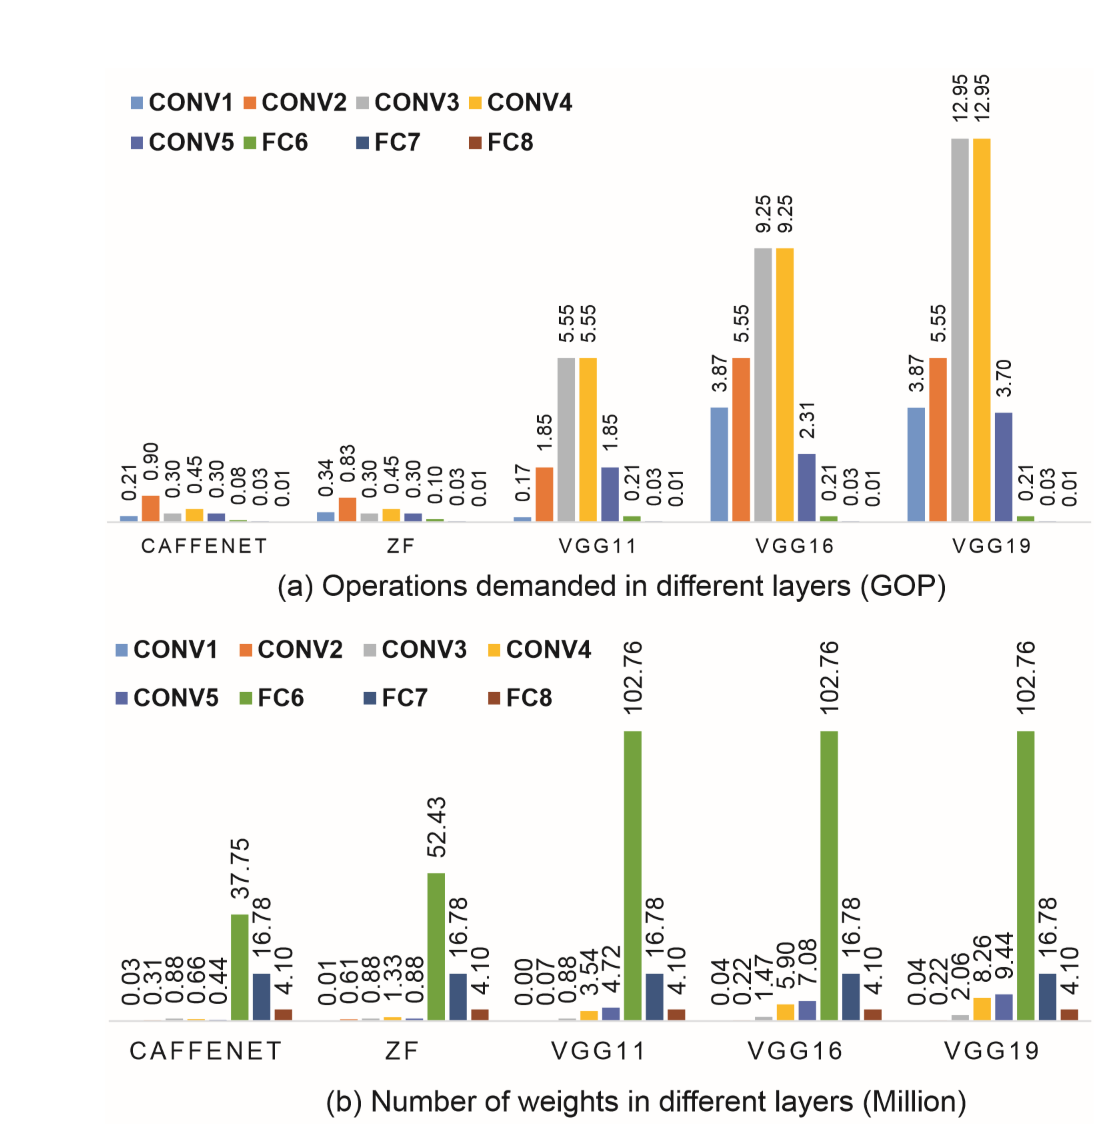
\includegraphics[width=0.7\textwidth]{complexityCNNModels.png} 
    \end{center}
    
    \caption{Complexity distribution of CNN models\\ \textbf{(Adopted figure from~\autocite{qiuGoingDeeperEmbedded2016})}}
    \label{fig:CNNcomplexity}   
\end{figure}

A significant portion of DNN computation is matrix-vector multiplication, ideally weight reuse techniques can speed up these operations.
However some DNNs feature FC layers with more than a hundred million weights (Fig.~\ref{fig:CNNcomplexity}), memory bandwidth here can be an issue since loading these weights can be a significant bottleneck~\autocite{qiuGoingDeeperEmbedded2016}. 
When the cache capacity is insufficient to store the weight matrix this bottleneck is expounded, causing memory accesses for every operation since the weight matrix cannot be reused~\autocite{hanEIEEfficientInference2016}.
As observed in Section~\ref{sec:MemAlloc} this indicates that compression techniques should help alliviate this bottleneck by making more parameters avaliable for cache reuse. The paper proposing EIE (an inference engine for compressed networks~\autocite{hanEIEEfficientInference2016}) shows that while compression does reduce the total number of operations, the irregular memory access patterns required when accessing sparse matrices mitigates improvements in inference performance, see Fig.~\ref{fig:wallClockEIE}.

\begin{figure}[H]
    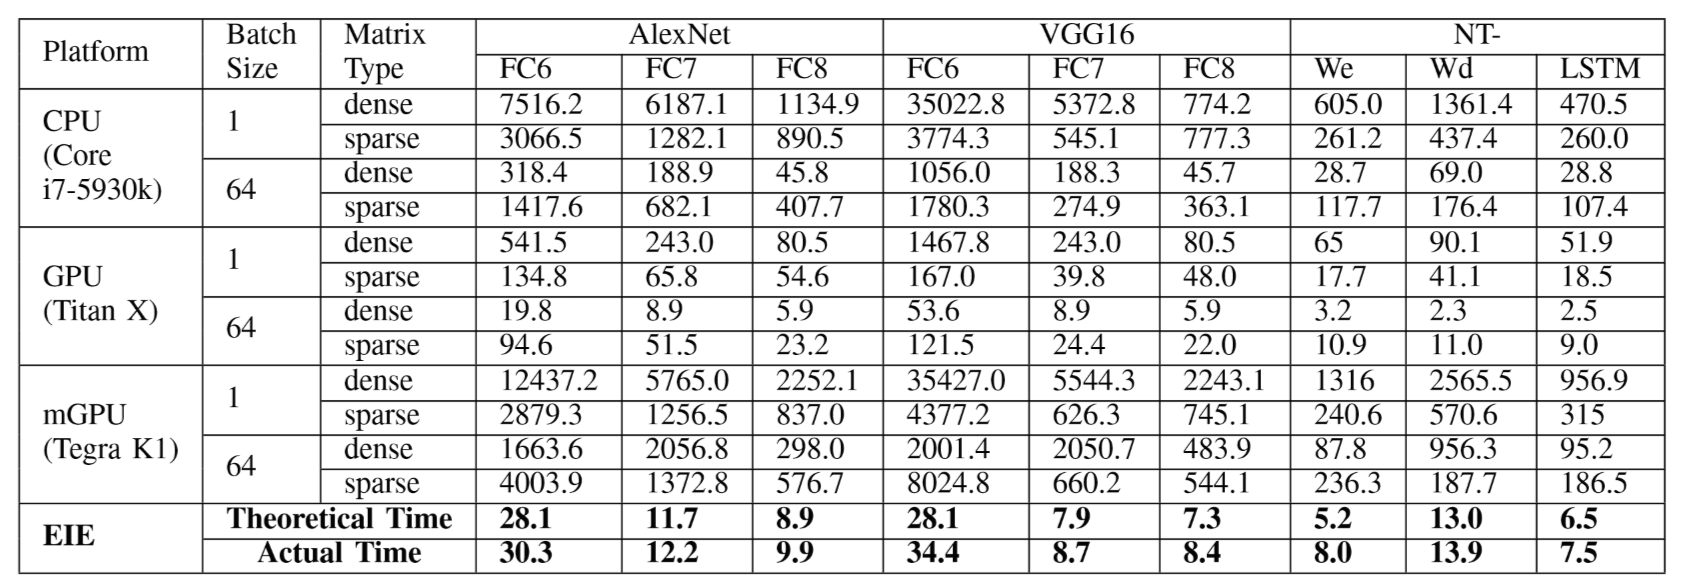
\includegraphics[width=1\textwidth]{wallClockEIE.png} 
    \caption{Wall clock time comparison for sparse and dense matrices between CPU, GPU, mGPU and EIE (an FPGA custom accelerator)\\ \textbf{(Adopted figure from~\autocite{hanEIEEfficientInference2016})}}
    \label{fig:wallClockEIE}   
\end{figure}

 Han et al~\autocite{hanEIEEfficientInference2016} provide a clear description of a technique for exploiting the sparity of activations by storing an encoded sparse weight matrix in a variant of compressed sparse column format~\autocite{vuducAutomaticPerformanceTuning}.

\end{document}